\newpage
\section{Analysis of Experimental Results}
\label {sec:results}

In what follows we introduce the following notation to refer to the different experiments performed. Let $\Sigma= (g, s(k, p), f, c)$ represent the execution of an experiment where:
\begin{itemize}
    \item $g$ is a datagraph;
    \item $s(k,p)$ represents a stream of transactions of length $k$ and percentage $p$ of anomalous transactions;
    \item $f$ is the number of filters;
    \item $c$ is the number of cores.
\end{itemize}

We perform experiments for: 
\begin{itemize}
    \item $g = $ \smallG\ and \mediumG;
    \item $s(k,p)$: 
    \begin{itemize}
        \item With $g = $ \smallG\ for $k=30, 60, 120$ and $p=0.02$.
        \item With $g = $ \mediumG\ for $k=7, 15$ and $p=0.03$.
    \end{itemize}
    \item $f$: 
    \begin{itemize}
        \item With $g = $ \smallG\ for $f=1,2,5,10,20,40,100,200,500,1000,2000$.
        \item With $g = $ \mediumG\ for $f=1,5,10,100,250,500,1000,2000,5000,10000$.
    \end{itemize} 
    \item $c = 1, 2, 4, 8, 16$
\end{itemize}

For instance, $\Sigma(\mathsf{GDB_A}, s(30, 0.02), f, c)$ refers to the experiment performed with $g = $ \smallG, $k=30$ days stream length and $p=0.02$ anomalous ratio, performed for all the filters $f$ combinations possible for $g = $ \smallG, and for all cores $c$ combinations.\\

\subsection*{E1: Evaluation in a High-Load Stress Scenario}

% Introducción
The evaluation of the \DPATM\ in this scenario was done for the two different bank databases; \smallG\ and \mediumG. 
For each simulated bank database system we provided the transactions streams that we generated. T
he details on the generated datasets are explained on \ref{exps:considered-datasets}. 
Let the Tables \ref{table:bank-dbs-details-again} and \ref{table:stream-sizes-again} serve as a summary.

\begin{table}[H]
\centering
\begin{tabular}{|c|c|c|c|c|}
\hline
\textbf{Name} & \textbf{$|\text{Card}|$} & \textbf{$|\text{ATM}|$} & \textbf{$|\text{ATM}_{\text{Internal}}|$} & \textbf{$|\text{ATM}_{\text{External}}|$} \\ \hline
\smallG    & 2000      & 50     & 40        & 10        \\ \hline
\mediumG    & 500000      & 1000     & 900        & 100        \\ \hline
\end{tabular}
\caption{Bank databases characteristics}
\label{table:bank-dbs-details-again}
\end{table}

\begin{table}[H]
    \small 
    \hspace*{-1.2cm}
    \centering
    \begin{tabular}{|l|c|c|c|c|c|c|}
    \hline
    \textbf{Name} & \textbf{Bank DB} & \textbf{$|\text{Days}|$} & \begin{tabular}[c]{@{}c@{}}\textbf{Anomalous}\\ \textbf{Ratio}\end{tabular} & \textbf{Stream Size} & \textbf{$|\text{Regular Tx}|$} & \textbf{$|\text{Anomalous Tx}|$} \\ \hline
    $\mathsf{GDB_A\text{-}30}$ & \smallG    & 30       & $0.02\ (2\%)$   & 39959       & 39508      & 451   \\ \hline
    $\mathsf{GDB_A\text{-}60}$ & \smallG     & 60       & $0.02\ (2\%)$   & 80744       & 79005      & 1739         \\ \hline
    $\mathsf{GDB_A\text{-}120}$ & \smallG     & 120      & $0.02\ (2\%)$   & 160750      & 157756     & 2994         \\ \hline
    $\mathsf{GDB_B\text{-}7}$ & \mediumG    & 7        & $0.03\ (3\%)$   & 2428286     & 2401806    & 26480        \\ \hline
    $\mathsf{GDB_B\text{-}15}$ & \mediumG    & 15       & $0.03\ (3\%)$   & 4856573     & 4805920    & 50653        \\ \hline
    \end{tabular}
    \caption{ \label{table:stream-sizes-again}Summary of the different streams generated for each of the bank databases. For each stream, we indicate the time interval (in days) that it simulates, the anomalous ratio, its exact stream size (in the number of transactions), and from it, its number of regular and only anomalous transactions.}
\end{table}

For each bank \DPATM\ system to be tested, we considered different \DPATM\ configurations 
regarding the number of filters with which we construct the \DP\ pipeline. 
This is controlled by setting up the system parameter \emph{maxFilterSize}, which determines the maximum number of cards each \filter\ stage tracks. 
Table \ref{table:exps-filters-variations} represents the different \emph{maxFilterSize} configurations tested for each of the bank systems.\\

Each of these \DPATM\ configurations were run for different resources variations in terms of the dedicated number of cores, 
in particular for $c = $\texttt{1}, \texttt{2}, \texttt{4}, \texttt{8} and \texttt{16} cores. 
For each particular number of cores setting the \DPATM\ configurations were compared against a sequential baseline version of our system (cores = \texttt{1}). 
This sequential version is referred in the following results as both the \textit{sequential/baseline} or as the \texttt{0-filter} version. 
It is a simple program version of the \DPATM\ that executes the same algorithm but without a \DP, that is, only with a main process that process the transactions one after the other tracking the activity of all the cards at once. It also implements the same stream ingestion method as the one referred in \ref{exps-input-reading}. However, it is different from the \DPATM\ with one single \filter\ stage in the sense that, this last contains a proper \filter\ \F\ stage with its respective \filterworker\ \FW\ substage, as well as a \source\ \Sr\ and a \sink\ \Sk\ stage.

\begin{table}[H]
    \renewcommand{\arraystretch}{1.5} % control row height
    \centering
    \begin{minipage}{0.45\textwidth}
        \centering
        \begin{tabular}{|c|c|}
        \hline
        \begin{tabular}[c]{@{}c@{}}\textbf{$|\text{Cards}|$ per \filter }\\ (\emph{maxFilterSize})\end{tabular} & \textbf{$|\text{\emph{Filter}}|$} \\ \hline
        2000   &   1     \\ \hline
        1000   &   2     \\ \hline
        400 &   5     \\ \hline
        200  &   10     \\ \hline
        100 &   20    \\ \hline
        50  &   40    \\ \hline
        20  &   100    \\ \hline
        10  &   200    \\ \hline
        4  &   500    \\ \hline
        2  &   1000    \\ \hline
        1  &   2000    \\ \hline
        \end{tabular}
        \caption*{\smallG}
    \end{minipage}
    \hfill
    \begin{minipage}{0.45\textwidth}
        \centering
        \begin{tabular}{|c|c|}
        \hline
        \begin{tabular}[c]{@{}c@{}}\textbf{$|\text{Cards}|$ per \filter }\\ (\emph{maxFilterSize})\end{tabular} & \textbf{$|\text{\emph{Filter}}|$} \\ \hline
        500000   &   1     \\ \hline
        100000   &   5     \\ \hline
        50000 &   10     \\ \hline
        5000  &   100     \\ \hline
        2000 &   250    \\ \hline
        1000  &   500    \\ \hline
        500  &   1000    \\ \hline
        250  &   2000    \\ \hline
        100  &   5000    \\ \hline
        50  &   10000    \\ \hline
        10  &   50000    \\ \hline
        \end{tabular}
        \caption*{\mediumG}
    \end{minipage}
    \caption{For \smallG\  and \mediumG, the different \DPATM\ configurations combinations for the \emph{maxFilterSize} parameter, including the derived number of \filter\ stages of the \DPATM.}
    \label{table:exps-filters-variations}
\end{table}

Each job was run ten times in the case of the experiments of the \smallG\ and one in the case of the \mediumG\ experiments, due to time constraints and its longer execution times. We limited to \texttt{16}GB of RAM the amount of memory used for each experiment. Note that in the case of the \mediumG, the tests with 50000 filters could not be performed due to this memory limitation.

% 1. Is it worthy the DPATM
\subsubsection*{\DPATM\ Comparison to Sequential Baseline}

First we provide and study the results to compare our different \DPATM\ configurations (with the different number of filters variations) with respect to the sequential version of the program, the \texttt{0-filter} version.\\

In Figure \ref{img:exps-small-120-combined} we can see the comparison of different metrics results for the experiment $\Sigma(\mathsf{GDB_A}, s(120, 0.02), f, c)$. We can see that the performance of the sequential version is, in general, the worst regarding all the metrics except for the Mean Response Time (\texttt{MRT}), where the \texttt{0-filter} exhibits a lower \texttt{MRT} than many configurations of the \DPATM, no matter the number of cores (\ref{fig:exps-small-120-mrt}).\\

In this sense, the sequential version achieves a lower \texttt{MRT} for any configuration with a number of filters above 40. Only the variations with a number of filters in the range 5-20 are able to outperform the sequential version on this metric, showing a \texttt{MRT} around 5-6 seconds in the 5 and 10 filter cases, for all the number of cores tested. To get more insights on this, we show in Figure \ref{img:exps-small-120-traces-reduced} the Response Time (\texttt{RT}) trace of the different configurations run with \texttt{16} cores. On it, as mentioned, we can see that only the configurations with a number of filters in the range 5-20 tend to have a \texttt{RT} below the sequential version for all of the checks. The 1-filter version is always above. However, an interesting phenomena that we see is that for the versions with 40 and more filters the \texttt{RT} presents a linear growing shape, whereas for the other versions the \texttt{RT} tends to be constant for all the performed checks. These \textit{large} number of filters versions even present a lower \texttt{RT} up to a certain number of checks. Later we will come again to this discussion, so to analyze better why this could be the cause of this behavior.
\\ 

Nevertheless, as expected, the sequential version underperforms for the other metrics such as the
Execution Time \texttt{ET} (\ref{fig:exps-small-120-et}), the throughput \texttt{T} (\ref{fig:exps-small-120-t}) and the \texttt{dief@t} (\ref{fig:exps-small-120-dieft}). In Figure \ref{img:exps-small-120-radar-dieft} we show the comparison of all these metrics together with a radar plot for the experiment $\Sigma(\mathsf{GDB_A}, s(120, 0.02), f, 16)$. A similar behavior can be observed in the experiments done for \mediumG. In Figure \ref{img:exps-medium-7D-radar-dieft}, we show the radar plot of the $\Sigma(\mathsf{GDB_B}, s(7, 0.03), f, 16)$ experiment. On it, again, only the versions with a number of filters in the range 5-20 outperform the sequential version in the \texttt{MRT}. However, for the rest of the metrics we can observe that, in general, almost all \DPATM\ configuration exhibits a better performance than the sequential version. \\


\begin{figure}[H]
    \centering
    \hspace*{-3cm} % Move content to the left
    \begin{subfigure}{0.5\textwidth}
        \centering
        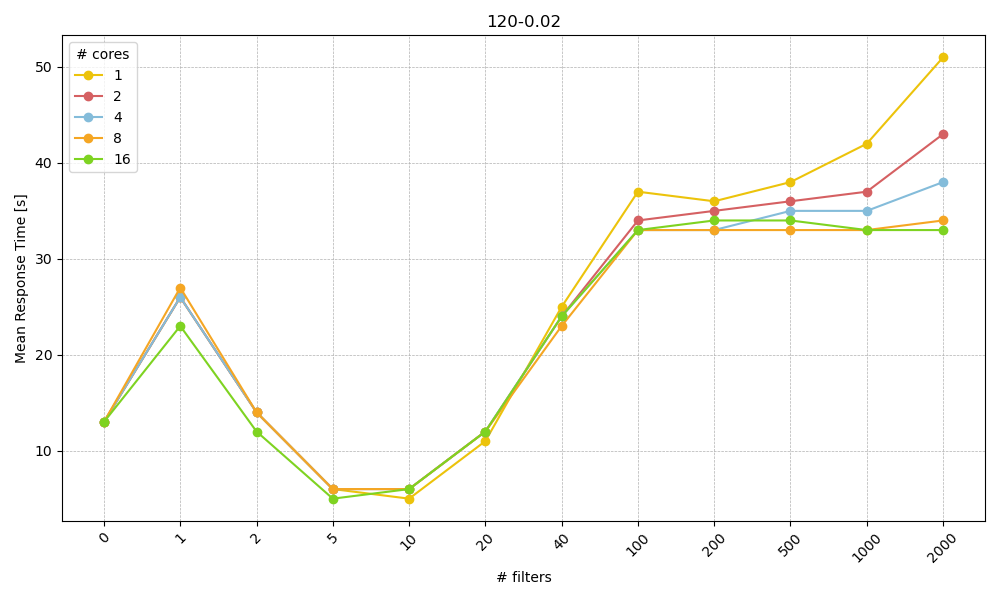
\includegraphics[scale=0.4]{images/4-Experiments/NRT/small/120-0.02/combined/mrt-1.png}
        \caption{Mean Response Time \texttt{MRT} (in seconds)}
        \label{fig:exps-small-120-mrt}
    \end{subfigure}
    \hspace{0.16\textwidth}
    \begin{subfigure}{0.5\textwidth}
        \centering
        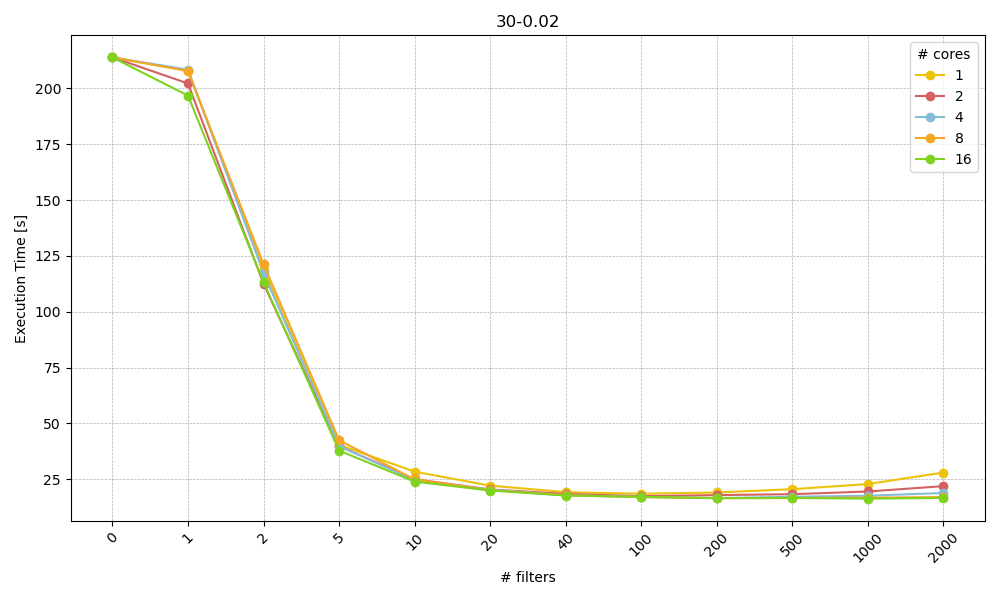
\includegraphics[scale=0.4]{images/4-Experiments/NRT/small/120-0.02/combined/execTime-1.png}
        \caption{Execution Time \texttt{ET} (in seconds)}
        \label{fig:exps-small-120-et}
    \end{subfigure}
    
    \vspace{0.5cm} % Vertical space between rows

    \hspace*{-3cm} % Move content to the left for the second row
    \begin{subfigure}{0.5\textwidth}
        \centering
        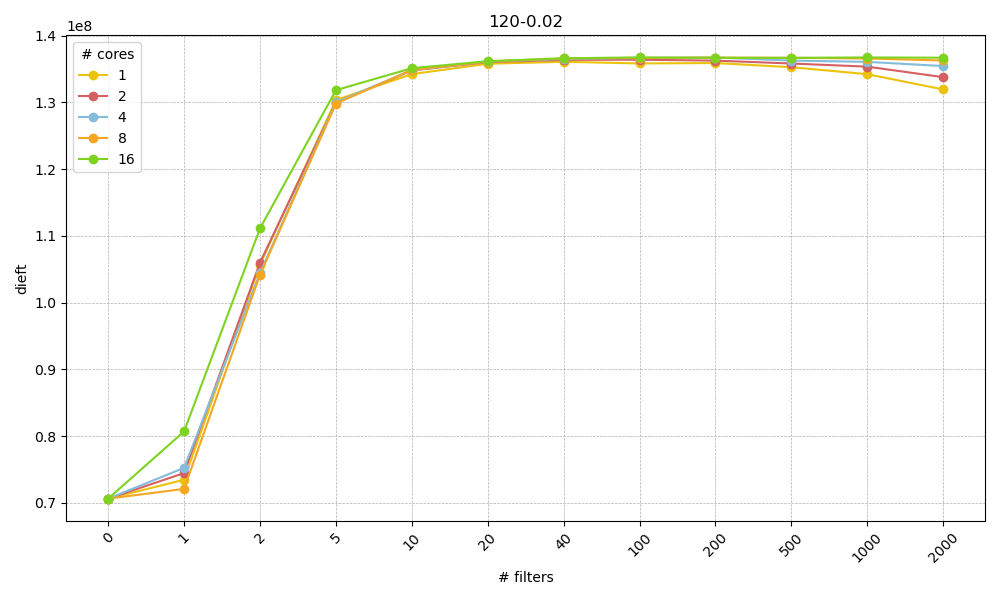
\includegraphics[scale=0.4]{images/4-Experiments/NRT/small/120-0.02/combined/dieft-1.png}
        \caption{\texttt{dief@t}}
        \label{fig:exps-small-120-dieft}
    \end{subfigure}
    \hspace{0.16\textwidth}
    \begin{subfigure}{0.5\textwidth}
        \centering
        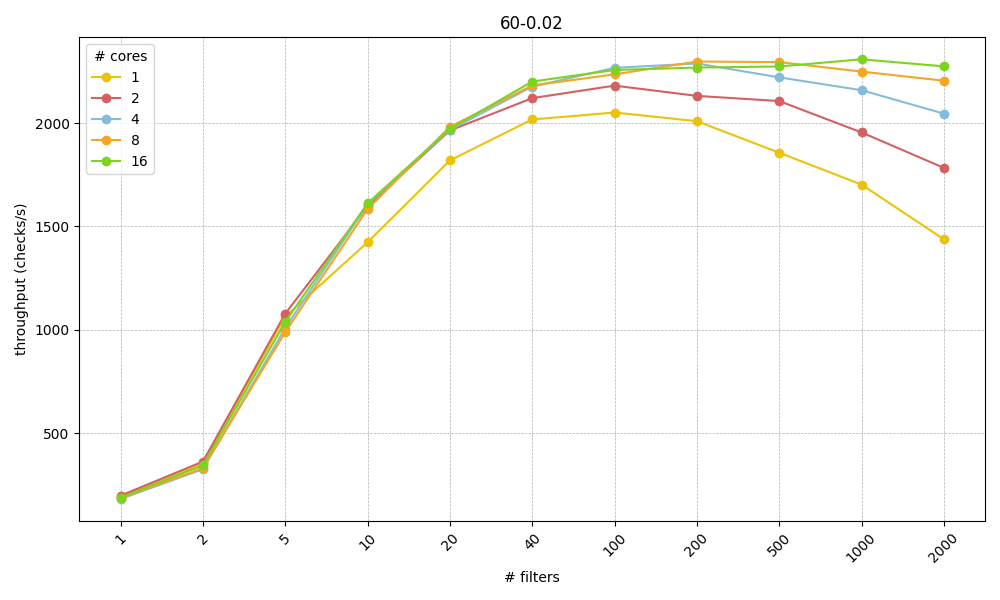
\includegraphics[scale=0.4]{images/4-Experiments/NRT/small/120-0.02/combined/throughput-1.png}
        \caption{Throughput \texttt{T} (checks/s)}
        \label{fig:exps-small-120-t}
    \end{subfigure}

    \caption{Metrics comparison for experiment $\Sigma(\mathsf{GDB_A}, s(120, 0.02), f, c)$. Each color represents the experiment run with a different number of cores.
    (a) \texttt{MRT}, (b) \texttt{ET}, (c) \texttt{dief@t}, (d) \texttt{T}.}
    \label{img:exps-small-120-combined}
\end{figure}

\begin{figure}[H]
    \centering
    \includegraphics[scale=0.6]{images/4-Experiments/NRT/small/120-0.02/fixedcores/16c/traces-response-time-reduced.png}
    \caption{Response Time (\texttt{RT}) trace for the $\Sigma(\mathsf{GDB_A}, s(120, 0.02), f, 16)$ test. Horizontal axis shows the \emph{check} number and the vertical axis shows the \texttt{RT} (in seconds) for that check.}
    \label{img:exps-small-120-traces-reduced}
\end{figure}

\begin{figure}[H]
    \centering
    \includegraphics[scale=0.6]{images/4-Experiments/NRT/small/120-0.02/fixedcores/16c/radar-dieft.png}
    \caption{Metrics radar plot comparison for the $\Sigma(\mathsf{GDB_A}, s(120, 0.02), f, 16)$ experiment. Each axis represents a metric: \texttt{MRT$^{-1}$}, \texttt{T} (Throughput), \texttt{dief@t}, \texttt{TFFT$^{-1}$} and \texttt{ET$^{-1}$}. Better performance for a metric is achieved whenever the value is closer to the outer boundary of the corresponding axis.}
    \label{img:exps-small-120-radar-dieft}
\end{figure}

\begin{figure}[H]
    \centering
    \includegraphics[scale=0.6]{images/4-Experiments/NRT/medium/7-0.03/fixedcores/16c/radar-dieft.png}
    \caption{Metrics radar plot comparison for the $\Sigma(\mathsf{GDB_B}, s(7, 0.03), f, 16)$ experiment. Each axis represents a metric: \texttt{MRT$^{-1}$}, \texttt{T} (Throughput), \texttt{dief@t}, \texttt{TFFT$^{-1}$} and \texttt{ET$^{-1}$}. Better performance for a metric is achieved whenever the value is closer to the outer boundary of the corresponding axis.}
    \label{img:exps-medium-7D-radar-dieft}
\end{figure}

\subsubsection*{Analysis of the Number of Filters Configuration}

Regarding the configuration of the \DPATM\ system, we are interested in analyzing which is the best configuration in terms of the number of filters for each the \smallG\ and \mediumG, given a certain number of cores resource limitation.\\

% smallG 
For \smallG, as already mentioned for the $\Sigma(\mathsf{GDB_A}, s(120, 0.02), f, c)$ test, regarding the \texttt{MRT} the configurations using 5-10 number of filters exhibit the best \texttt{MRT}, of around 5-6 seconds, worsening for the configurations with a large number of filters (see Figure \ref{fig:exps-small-120-mrt}). Indeed they show a constant and low response time in comparison with the ones with large number of filters; see Figure \ref{fig:exps-small-120-et}.\\

Nonetheless, these configurations do not perform that well in the case of the \ET\ or the \dieft, where a larger number of filters seems to be a better option, being able to consume the input stream faster and showing a better continuous behavior in terms of \dieft. However, it is worthy to note that the behavior tends to degrade for all the metrics in the case of having a low number of cores. We can see this clearly for the case of the runs with \texttt{1} core. It can be seen that, in this case, a large number of filters could be causing an overhead and therefore producing this degradation of the behavior for the \ET\ and the \dieft. We can observe this in all the metrics figures of Figure \ref{img:exps-small-120-combined}, where specially for the \texttt{1} core variations, we can appreciate the degradation for the large number of filters configurations (in the rightmost part of each of the plots). As expected, more cores help to improve the behavior, especially for the variants with large number of filters.\\

The analysis on the number of filters configuration is quite similar in the case of the experiments done for \mediumG. For instance, in Figure \ref{img:exps-medium-15D-8c-radar-dieft} we show the metrics radar for $\Sigma(\mathsf{GDB_B}, s(15, 0.03), f, 8)$, where we can also see that the configurations that achieve the best \MRT\ are the ones with a number of filters in the range 5-10, whereas they are the ones that underperform in the \ET\ and \dieft\ metrics. This can also be seen in the results trace of this same test on Figure \ref{img:exps-medium-15D-8c-trace}, where the continuous behavior for these filter configurations underperforms the continuous behavior for configurations with higher number of filters. However, they have a better continuous behavior than the sequential or the 1 filter configurations.\\

\begin{figure}[H]
    \centering
    \includegraphics[scale=0.6]{images/4-Experiments/NRT/medium/15-0.03/fixedcores/8c/radar-dieft.png}
    \caption{Metrics radar plot comparison for $\Sigma(\mathsf{GDB_B}, s(15, 0.03), f, 8)$. Each axis represents a metric: \texttt{MRT$^{-1}$}, \texttt{T} (Throughput), \texttt{dief@t}, \texttt{TFFT$^{-1}$} and \texttt{ET$^{-1}$}. Better performance for a metric is achieved whenever the value is closer to the outer boundary of the corresponding axis.}
    \label{img:exps-medium-15D-8c-radar-dieft}
\end{figure}

\begin{figure}[H]
    \centering
    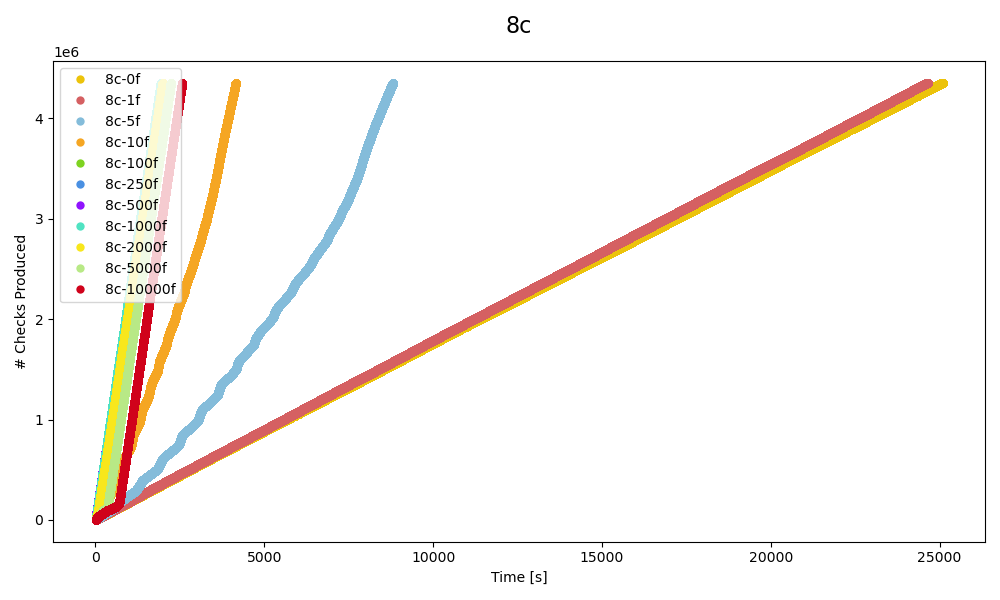
\includegraphics[scale=0.6]{images/4-Experiments/NRT/medium/15-0.03/fixedcores/8c/traces.png}
    \caption{Check results trace for $\Sigma(\mathsf{GDB_B}, s(15, 0.03), f, 8)$. Pairs (result, time(s)). Vertical axis shows the \emph{check} number and horizontal axis shows the time in seconds at which that check is produced.}
    \label{img:exps-medium-15D-8c-trace}
\end{figure}

Another aspect in which the configurations in the range of 5-10 number of filters outperform, apart from achieving the lowest \MRT\ is in achieving it through a constant \RT\ along all the execution. Figure \ref{img:exps-medium-15-rtraces-reduced} shows the response time trace for the $\Sigma(\mathsf{GDB_B}, s(15, 0.03), f, 8)$. On it, the 5-filter variant maintains a \RT\  around 11 seconds and the 10-filter around 9 seconds, in comparison to other larger number of filters variations that end up accumulating more than 100s of \RT.\\

\begin{figure}[H]
    \centering
    \includegraphics[scale=0.6]{images/4-Experiments/NRT/medium/15-0.03/fixedcores/8c/traces-response-time-reduced.png}
    \caption{Response Time (\texttt{RT}) trace for $\Sigma(\mathsf{GDB_B}, s(15, 0.03), f, 8)$. Horizontal axis shows the \emph{check} number and the vertical axis shows the \texttt{RT} (in seconds) for that check.}
    \label{img:exps-medium-15-rtraces-reduced}
\end{figure}

In addition, the degradation of the behavior of the configurations with a high number of filters for a low number of cores executions is a phenomena that we can also see in the \mediumG\ experiments. For instance we can see the degradation of the \ET\ in Figure \ref{img:exps-medium-7-et} in the case of the test $\Sigma(\mathsf{GDB_B}, s(7, 0.03), f, c)$. On it, we observe how the \ET\ deteriorates for the configurations with a high number of filters (2000, 5000 and 10000) whenever we reduce the number of cores. This can be due to: (i) an overhead on the number of \texttt{goroutines} utilized and the overhead in the communication of the pipeline that this might be causing; (ii) the overhead on the communication to the Neo4j graph database instance through those many parallel sessions, remember that we have one parallel session per filter stage; (iii) a bottleneck at the \sink \Sk\ stage, caused by its current file writing of the results. However, note that in a real implementation of the system the results emission would be done in another manner, such as the emission of the alerts through the network to the cardholder. In any case, further investigation and potential improvements to address this issue will be considered as future work.


\begin{figure}[H]
    \centering
    \hspace*{-1.7cm} % Move content to the left
    \begin{subfigure}{0.5\textwidth}
        \centering
        \includegraphics[scale=0.55]{images/4-Experiments/NRT/medium/7-0.03/fixedcores/1c/execTime.png}
        \caption{}
        \label{fig:exps-medium-7-mrt-1c}
    \end{subfigure}
    \hspace*{1cm} 
    \begin{subfigure}{0.5\textwidth}
        \centering
        \includegraphics[scale=0.55]{images/4-Experiments/NRT/medium/7-0.03/fixedcores/2c/execTime.png}
        \caption{}
        \label{fig:exps-medium-7-mrt-4c}
    \end{subfigure}

    \vspace{0.5cm} % Vertical space between rows

    \hspace*{-1.7cm} % Move content to the left for the second row
    \begin{subfigure}{0.5\textwidth}
        \centering
        \includegraphics[scale=0.55]{images/4-Experiments/NRT/medium/7-0.03/fixedcores/4c/execTime.png}
        \caption{}
        \label{fig:exps-medium-7-mrt-8c}
    \end{subfigure}
    \hspace*{1cm}
    \begin{subfigure}{0.5\textwidth}
        \centering
        \includegraphics[scale=0.55]{images/4-Experiments/NRT/medium/7-0.03/fixedcores/8c/execTime.png}
        \caption{}
        \label{fig:exps-medium-7-mrt-16c}
    \end{subfigure}

    \caption{\ET\ for $\Sigma(\mathsf{GDB_B}, s(7, 0.03), f, c)$. (a) Run with $c=$ \texttt{1} core. (b) Run with $c=$ \texttt{2} cores. (c) Run with $c=$ \texttt{4} cores. (d) Run with $c=$ \texttt{8} cores.}
    \label{img:exps-medium-7-et}
\end{figure}

% Enseñar el rt que permanece constante
% Sacar tabla con mrt para cada una de las variantes con 5,10,20f... o algo asi ->
% justificar que el dpatm con esta config es conveniente como real time system en este escenario... etc... HACER COMO UN CIERRE
Finally, since we consider \MRT\ one of the most important metrics for assessing the suitability of our \DPATM\ as a real-time system for the rapid detection of card-ATM fraud, we show Tables \ref{table:mrt-comparison-small-120} and \ref{table:mrt-comparison-medium-15} on which we show the \MRT\ values in seconds for the experiments performed on the \smallG\ and \mediumG\ largest tested streams, $k=120$ and $k=15$, respectively. On them we can show that, in the case of the $\Sigma(\mathsf{GDB_A}, s(120, 0.02), f, c)$ the best filter (5 and 10 filters) configuration has a \MRT\ around 5-6 seconds for all the tested number of cores variation. For the $\Sigma(\mathsf{GDB_B}, s(15, 0.03), f, c)$, the best filter configurations in this metric, again the 5 and 10 filter configurations, achieve a \MRT\ around 10 seconds.

\begin{table}[H]
    \centering
    \begin{tabular}{|c||c|c|c|c|c|}
        \hline
        \multicolumn{6}{|c|}{\textbf{MRT (s) for \smallGOneTwoZero}} \\
        \hline
        \multicolumn{6}{|c|}{Number of Cores} \\
        \hline
        \textbf{\# Filters} & \textbf{1} & \textbf{2} & \textbf{4} & \textbf{8} & \textbf{16} \\
        \hline
        $\mathsf{0}$     & 13  & 13  & 13  & 13  & 13  \\
         $\mathsf{1}$     & 26  & 26  & 26  & 27  & 23  \\
         $\mathsf{2}$     & 14  & 14  & 14  & 14  & 12  \\
         $\mathsf{5}$     & 6   & 6   & 6   & 6   & 5   \\
         $\mathsf{10}$    & 5   & 6   & 6   & 6   & 6   \\
         $\mathsf{20}$    & 11  & 12  & 12  & 12  & 12  \\
        $\mathsf{40}$   & 25  & 24  & 24  & 23  & 24  \\
         $\mathsf{100}$   & 37  & 34  & 33  & 33  & 33  \\
         $\mathsf{200}$   & 36  & 35  & 33  & 33  & 34  \\
        $\mathsf{500}$   & 38  & 36  & 35  & 33  & 34  \\
         $\mathsf{1000}$  & 42  & 37  & 35  & 33  & 33  \\
         $\mathsf{2000}$  & 51  & 43  & 38  & 34  & 33  \\
        \hline
    \end{tabular}
    \caption{Mean Response Time (\MRT) in seconds for the $\Sigma(\mathsf{GDB_A}, s(120, 0.02), f, c)$ experiment.}
    \label{table:mrt-comparison-small-120}
\end{table}


\begin{table}[H]
    \centering
    \begin{tabular}{|c||c|c|c|c|c|}
        \hline
        \multicolumn{6}{|c|}{\textbf{MRT (s) for \mediumGFifteen}} \\
        \hline
        \multicolumn{6}{|c|}{Number of Cores} \\
        \hline
        \textbf{\# Filters} & \textbf{1} & \textbf{2} & \textbf{4} & \textbf{8} & \textbf{16} \\
        \hline
         $\mathsf{0}$     & 13   & 13   & 13   & 13   & 13   \\
         $\mathsf{5}$     & 11   & 10   & 11   & 11   & 9    \\
         $\mathsf{10}$    & 11   & 9    & 10   & 9   & 7    \\
         $\mathsf{100}$   & 33   & 40   & 29   & 23   & 37   \\
         $\mathsf{250}$   & 124  & 80   & 91   & 69   & 90   \\
         $\mathsf{500}$   & 221  & 161  & 134  & 136  & 138  \\
         $\mathsf{1000}$  & 502  & 301  & 267  & 256  & 263  \\
         $\mathsf{2000}$  & 937  & 702  & 618  & 562  & 554  \\
         $\mathsf{5000}$  & 2830 & 1732 & 1422 & 1124 & 1060 \\
         $\mathsf{10000}$ & 4957 & 2535 & 2025 & 1410 & 1249 \\
        \hline
    \end{tabular}
    \caption{Mean Response Time (\MRT) in seconds for the $\Sigma(\mathsf{GDB_B}, s( 15, 0.03), f, c)$ experiment.}
    \label{table:mrt-comparison-medium-15}
\end{table}

% Pongo lo de las interactions per second y su plot
\begin{figure}[H]
    \centering
    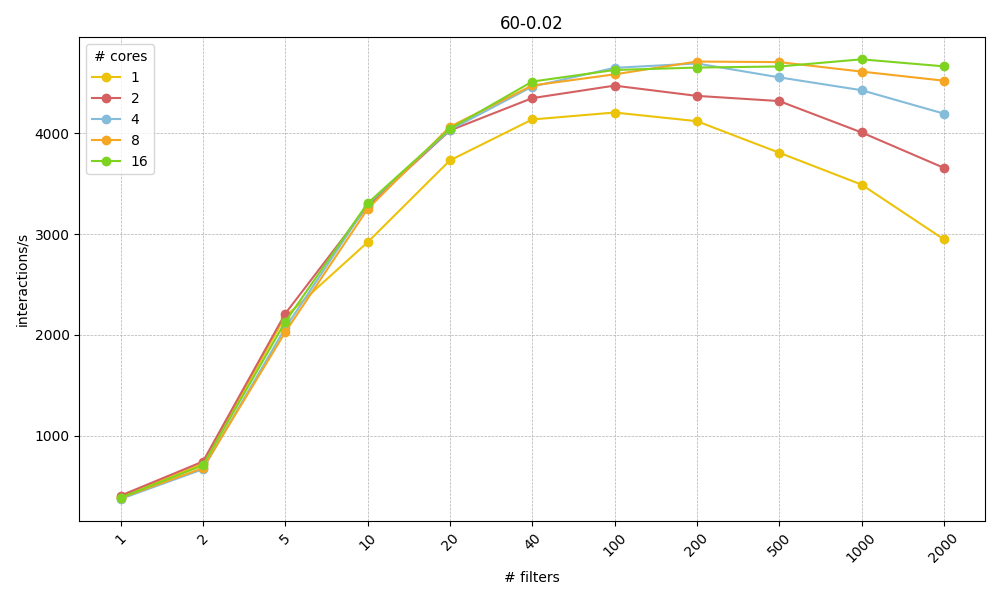
\includegraphics[scale=0.6]{images/4-Experiments/NRT/small/120-0.02/combined/interactions-1.png}
    \caption{Processed \texttt{interactions/s} on the experiment $\Sigma(\mathsf{GDB_A}, s(120, 0.02), f, c)$. Horizontal axis shows the variation in the number of filters $f$. Vertical axis shows the number of processed \texttt{interactions/s}. Each color represents the run with a different number of cores $c$.}
    \label{img:exps-small-120-interactions-new}
\end{figure}

% Mencionar el tradeoff
To sum up, we can say that there is a trade-off between \MRT\ and the other metrics. The \DPATM\ configurations that offer the best balance across all metrics are those with 5 to 10 filters. We reason that this is the case since, as we already discussed in \ref{exps-design-e1}, we consider that a real-time system in this high-load stress scenario needs to show a good performance in various aspects. First, have a low and non-increasing - if possible - response time, so to allow the user / bank system be able to prevent potential the current and future frauds as fast as possible. In this sense, these configurations achieve reasonable low \MRT\ times, in all the cases lower than 11 seconds. Secondly, they also have a reasonable good continuous behavior and have a good performance in terms of the speed to process the stream input. For instance, in $\Sigma(\mathsf{GDB_A}, s(120, 0.02), f, c)$ experiment, we are able to achieve a rate of almost 5,000 \texttt{interactions/s} (2,500 transactions/s) processed (see the Figure \ref{img:exps-small-120-interactions-new}).
Therefore, we conclude that these \DPATM\ configurations achieve a good balance across all these aspects.